\documentclass{standalone}
\usepackage{tikz}

\usetikzlibrary{calc,math}


\begin{document}

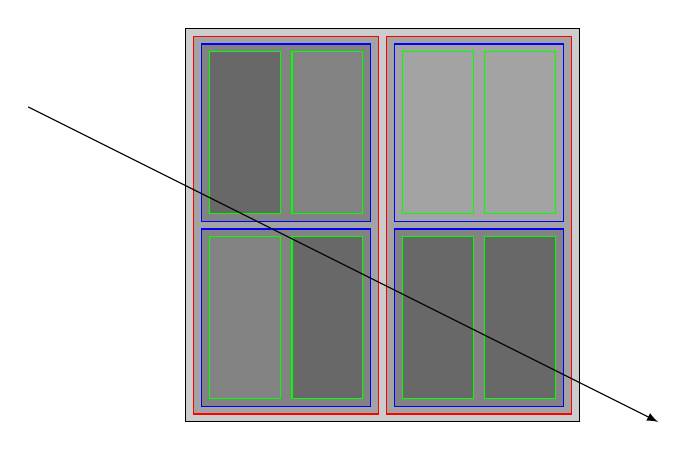
\begin{tikzpicture}
  \path[fill=black,opacity=0.2] (0,0) rectangle (5,5);

  \path[fill=black,opacity=0.2] (0.1,0.1) rectangle (2.45,4.9);
  \path[fill=black,opacity=0.2] (2.55,0.1) rectangle (4.9,4.9);

  \path[fill=black,opacity=0.2] (0.2,0.2) rectangle (2.35, 2.45);
  \path[fill=black,opacity=0.2] (0.2,2.55) rectangle (2.35,4.8);
  \path[fill=black,opacity=0.2] (2.65,0.2) rectangle (4.8, 2.45);

  \path[fill=black,opacity=0.2] (1.35,0.3) rectangle ++(0.9,2.05);
  \path[fill=black,opacity=0.2] (0.3,2.65) rectangle ++(0.9,2.05);
  \begin{scope}[xshift=2.45cm]
    \path[fill=black,opacity=0.2] (0.3,0.3) rectangle ++(0.9,2.05);
    \path[fill=black,opacity=0.2] (1.35,0.3) rectangle ++(0.9,2.05);
  \end{scope}

  \draw (0,0) rectangle (5,5);
  \draw[red] (0.1,0.1) rectangle (2.45,4.9);
  \draw[red] (2.55,0.1) rectangle (4.9,4.9);
  \draw[blue] (0.2,0.2) rectangle (2.35, 2.45);
  \draw[blue] (0.2,2.55) rectangle (2.35,4.8);
  \draw[blue] (2.65,0.2) rectangle (4.8, 2.45);
  \draw[blue] (2.65, 2.55) rectangle (4.8,4.8);
  \draw[green] (0.3,0.3) rectangle ++(0.9,2.05);
  \draw[green] (1.35,0.3) rectangle ++(0.9,2.05);
  \draw[green] (0.3,2.65) rectangle ++(0.9,2.05);
  \draw[green] (1.35,2.65) rectangle ++(0.9,2.05);

  \begin{scope}[xshift=2.45cm]
    \draw[green] (0.3,0.3) rectangle ++(0.9,2.05);
    \draw[green] (1.35,0.3) rectangle ++(0.9,2.05);
    \draw[green] (0.3,2.65) rectangle ++(0.9,2.05);
    \draw[green] (1.35,2.65) rectangle ++(0.9,2.05);
  \end{scope}
  
  \draw[-latex] (-2,4) -- (6,0);
\end{tikzpicture}

\end{document}